\documentclass[12pt,a4paper]{article}
\usepackage[a4paper,left=1.5cm,right=1.5cm,top=2.5cm,bottom=2.5cm]{geometry}
\usepackage{multicol}
\usepackage{caption}
\usepackage{graphicx}
\usepackage{float}
\usepackage{indentfirst}
\usepackage{tcolorbox}

\newenvironment{Figure}
{\par\medskip\noindent\minipage{\linewidth}}
{\endminipage\par\medskip}


%%%%%%%%%%%%%%%%%%%%%%%%%%%%%%%%%%%%%%%%%%%%%%%%%%%%%%%%%%%%%%%%%%%%%%%%%%%%%%%%%%%%%%%%%%%%%%%%%%%%%%%%%%%%%


\begin{document}

	\title{Rapport de projet -- Programmation Orientée Objet}
	\author{Damien \textsc{Garcia} -- Florian \textsc{Echelard}}
	\date{Novembre 2022}
	
	\begin{tcolorbox}
		\maketitle		
	\end{tcolorbox}


%%%%%%%%%%%%%%%%%%%%%%%%%%%%%%%%%%%%%%%%%%%%%%%%%%%%%%%%%%%%%%%%%%%%%%%%%%%%%%%%%%%%%%%%%%%%%%%%%%%%%%%%%%%%%

	
	\begin{multicols}{2}

		\section{Introduction}

		Le but de ce projet est de fournir un outil de gestion de radiographies pour les médecins au sein d'un centre de santé en s'appuyant sur le paradigme de programmation orienté objet. Pour cela, nous avons commencé par établir les objectifs d'ergonomie et d'accessibilité relatifs à ce logiciel, discuté ensuite de l'implémentation en classes et leur interface relationnelle, puis des éléments utilisés au niveau du code pour élargir et préciser l'application.
		
		
%%%%%%%%%%%%%%%%%%%%%%%%%%%%%%%%%%%%%%%%%%%%%%%%%%%%%%%%%%%%%%%%%%%%%%%%%%%%%%%%%%%%%%%%%%%%%%%%%%%%%%%%%%%%%


		\section{Objectifs et Approche}
		
		L'interface définie par le projet doit permettre à un médecin d'accéder aux radiographies de ses patients, ainsi qu'aux données associées à ces radiographies. Un médecin donné, n'aura accès qu'aux radiographies de ses propres patients, mais pas à celles des autres médecins.\\
				
		Du fait de la séparation des accès aux données, des méthodes de recherches, autorisant ou non l'accès à celles-ci doivent être établies et implémentées. De plus certaines de ces données doivent être protégée par mot de passe, notamment le rapport médical associé aux examens médicaux. Dans un objectif de cohérence générale de l'implémentation, nous avons rapidement opté par implémenter un système de \textit{Login}, c'est-à-dire qu'un utilisateur, avant de pouvoir accéder à quelconque donnée, doit s'identifier sur la base de données ce qui permettra par la suite de lui rendre disponible uniquement les dossiers médicaux lui étant associés. \\
				
		Ces différents niveaux d'accessibilité variant les informations qu'un utilisateur peut recevoir, le premier réflexe était de regrouper les éléments d'intérêt dans un classe à l'interface des utilisateurs et de l'accès à la base de données pour distribuer de manière contrôlée les attributs. \\
				
		Nous avons cependant changé cette considération ensuite pour inclure l'interface et la gestion de la base de donnée dans une entité pouvant faire appel aux éléments utilisateurs lors d'une session. \\
				
		Le changement de paradigme s'est opéré quant nous avons implémenté un autre critère du cahier des charges qui nous a été donné, la sauvegarde des données entre les sessions d'accession. Cette approche de \textit{serializing} nous permettait de concevoir l'application en deux états, active et inactive. A l'activation, les données sont téléchargées (\textit{download}), et à la sortie du logiciel sauvegardées (\textit{upload}). \\
				
		L'interface (faisant référence ici au visuel de l'application, le \"menu\") ayant accès aux méthodes de la base de données comme détaillé ici-bas, une classe faisant le lien entre utilisateur et radiographie n'était plus nécessaire, tous deux existant dans la même entité instanciée, la \textbf{session}.
		
		
%%%%%%%%%%%%%%%%%%%%%%%%%%%%%%%%%%%%%%%%%%%%%%%%%%%%%%%%%%%%%%%%%%%%%%%%%%%%%%%%%%%%%%%%%%%%%%%%%%%%%%%%%%%%%
				
				
		\section{Implémentation}
				
		La volonté de proposer plusieurs profils pour ouvrir cette application non seulement au corps médical, mais aux patients, nous a motivé à créer une classe parent \textbf{User}, qui comporte les renseignements généraux, soit le nom, le prénom, et le mot de passe. Là réside une des différences avec le cahier des charges, qui demandait uniquement une sécurisation des images de radiographie. L'accès à un profil utilisateur ne peut se faire uniquement que si les informations fournies (\textbf{id, mot de passe}) correspondent à celles présentes dans la base de données. \\
				
		Notre application se sert du statut docteur reconnu dans la base de données pour fournir une session complète, soit la liste des patients, et la recherche d'un patient précis donne accès aux méthodes de recherche par date et numéro d'examen. Le patient lui n'a accès qu'à la deuxième partie, étant donné qu'il ne doit que voir ses propres examens. Il a cependant accès aux méthodes de recherche par date et par idientifiant de radiographie.\\
				
		Lors de n'importe laquelle session, selon le niveau, différentes informations sont affichées. Ces informations sont actualisées en temps réel par des méthodes d'actualisation de la base de données, ce qui permet que lors de l'appel des méthodes d'ajout et de suppression des patients, des radiographies associées à un patient, et des \textit{snapshots} ou images radiographiques, l'ajout est visible en temps réel.\\
				
		Les utilisateurs héritant de la classe \textbf{User} sont donc \textbf{Docteur} et \textbf{Patient}, qui sont gérés dans la classe \textbf{\textit{Database\_Handling}} ou \textbf{DBH}, et instanciés temporairement dans la classe \textbf{Interface}, ils composent donc la gestion de la base de donnée, et par extension, la session. \\
				
		\textbf{DBH} utilise une méthode de serializing simple itérant sur les lignes d'un fichier texte pour y associer les variables à implémenter dans la classe \textbf{Radiographie}. \textbf{Interface} hérite donc de \textbf{DBH} et cette dernière est composée de radiographies.
				
		La classe \textbf{Interface} permet de proposer un menu intéractif affichant le contenu chargé par \textbf{DBH} au lancement de la session, ainsi que l'actualisation de l'information.
		
	\end{multicols}
	
%	\pagebreak

	\begin{figure}[H]
		\centering
		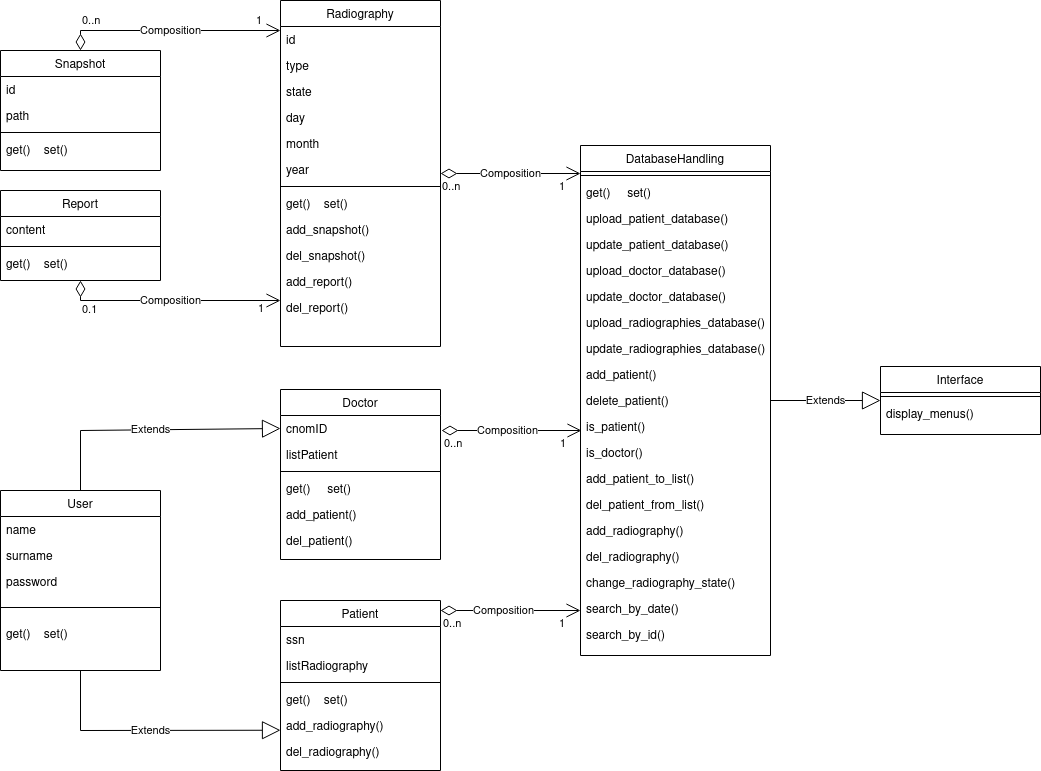
\includegraphics[width=0.8\linewidth]{images/UML_OOP.png}
		\captionof{figure}{Diagramme UML présentant la structure de l'implémentation}
		\label{fig:UML}
	\end{figure}

	\pagebreak


%%%%%%%%%%%%%%%%%%%%%%%%%%%%%%%%%%%%%%%%%%%%%%%%%%%%%%%%%%%%%%%%%%%%%%%%%%%%%%%%%%%%%%%%%%%%%%%%%%%%%%%%%%%%%


	\begin{multicols}{2}
		
		\section{Utilisation de l'interface}
				
		Avec de faux docteurs et patients, ainsi que des radiographies, déjà présent dans notre jeu de données, nous allons procéder à un test de notre application. \\
				
		Pour commencer, voici comment le menu principal se présente au lancement de l'application (Figure 1). \\
		\begin{Figure}
			\centering
			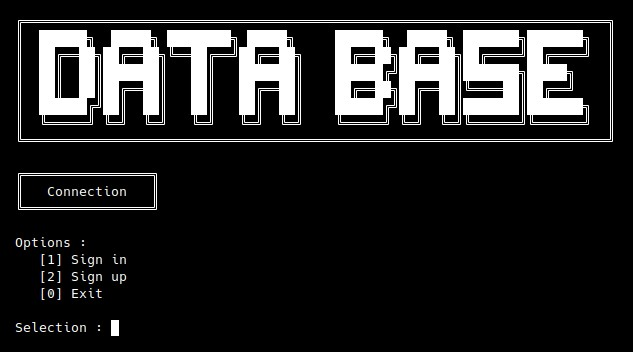
\includegraphics[width=\linewidth]{images/walkthrough/entree.jpg}
			\captionof{figure}{Menu principal}
			\label{fig:menu_principal}
		\end{Figure}
				
		Si l'on choisit de s'inscrire, une invite se présente donnant 3 tentatives avant de revenir au menu principal, comme présenté dans la Figure 2.
				

		\begin{Figure}
			\centering
			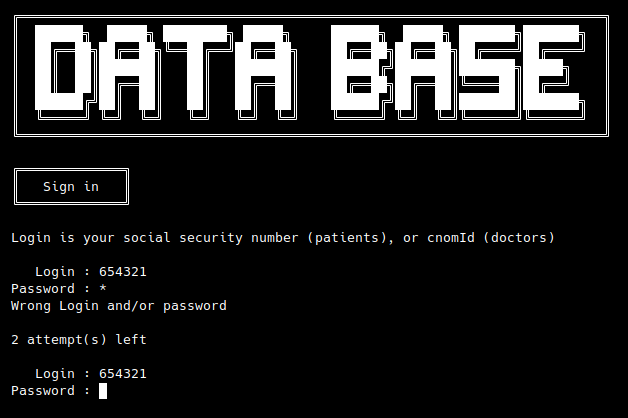
\includegraphics[width=\linewidth]{images/walkthrough/sign_in.png}
			\captionof{figure}{Menu principal}
			\label{fig:page_connexion}
		\end{Figure}		

		Ici, nous fournissons l'information d'un docteur, il est donc reconnu et nous pouvons accéder à sa liste de patient, ainsi que l'accès à un patient précis, l'ajout et la délétion de patients, comme vu dans la Figure 3.
					

		\begin{figure}
			\centering
			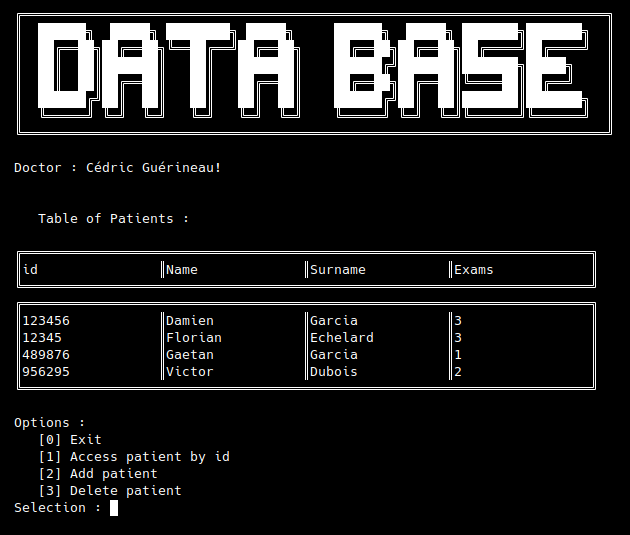
\includegraphics[width=\linewidth]{images/walkthrough/doctor_main.png}
			\captionof{figure}{Liste de patients du menu Docteur}
			\label{fig:menu_docteur}
		\end{figure}
				
		Si l'on décide d'accéder à un patient grâce à un identifiant, un nouveau menu s'affiche, avec la liste des radiographies que cet individu a effectué. Nous pouvons décider de regarder le contenu d'une consultation, que ce soit par un identifiant précis ou la date de consultation. Nous pouvons aussi tenter de rentrer une nouvelle consultation pour ce patient, ce que nous allons essayer de suite dans la Figure 4.
				
		\begin{figure}
			\centering
			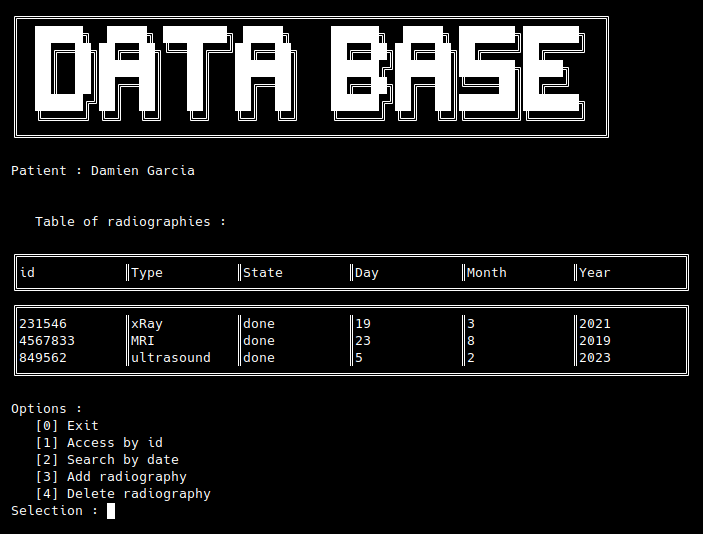
\includegraphics[width=\linewidth]{images/walkthrough/doctor_patient_main.png}
			\captionof{figure}{Le menu spécifique pour un patient}
			\label{fig:menu_patient}
		\end{figure}

	\end{multicols}
	
\end{document}